\documentclass[12pt]{article}
\usepackage[utf8]{inputenc}
\usepackage{amsmath}
\usepackage{multicol}
\usepackage{graphicx}
\usepackage{float}
\usepackage{dsfont}
\usepackage{textcomp}
\usepackage[center]{caption}
\usepackage{caption}
\usepackage{siunitx}
\usepackage{amsfonts}
\usepackage{hyperref}
\usepackage{amsmath}
\usepackage{csquotes}
\usepackage[style=authoryear,backend=biber]{biblatex}
\addbibresource{mybib.bib}
\hypersetup{
    colorlinks,
    citecolor=black,
    filecolor=black,
    linkcolor=black,
    urlcolor=black
}
\usepackage{cleveref}
\usepackage{fancyhdr}
\setlength{\headheight}{14.5pt}
\renewcommand\theContinuedFloat{\alph{ContinuedFloat}}
\renewcommand{\sectionmark}[1]{\markright{#1}{}}
\usepackage[T1]{fontenc}
\usepackage[colorinlistoftodos]{todonotes}
\usepackage[margin=2cm,a4paper]{geometry}
\newgeometry{left=1.5cm,right=1.5cm,top=2.0cm,bottom=2.0cm}
\usepackage{listings}
\setlength{\marginparwidth}{2cm}
\setlength{\parindent}{14pt}
\newcommand{\deriv}{\mathrm{d}}
\title{}
\pagestyle{fancy}
\fancyhf{}
\rhead{Section \thesection}
\lhead{Assignment 4: Spectroscopy}
\lfoot{PH512: Data Analysis Techniques in Astronomy and Planetary Science}
\rfoot{Page \thepage}
\renewcommand{\headrulewidth}{1pt}
\renewcommand{\footrulewidth}{1pt}


\begin{document}
\begin{titlepage}
\newgeometry{left=1.0in,right=1.0in,top=0.8in,bottom=0.8in}
\newcommand{\HRule}{\rule{\linewidth}{0.5mm}}
\begin{centering} 

%---------------------------------------------------------------------------
%	TITLE SECTION
%---------------------------------------------------------------------------

\includegraphics[scale=0.7]{Images/Uni_of_Kent.png}\\[0.3cm]
\HRule \\ [0.3cm]
\Huge{\bfseries{Spectroscopy}} \\
\textsc{\large Data Analysis Techniques in Astronomy and Planetary Science}\\ [-0.1cm]
\textsc{\large BSc(Hons) Astronomy, Space Science and Astrophysics}\\ [-0.2cm]
\HRule \\[0.5cm]
%---------------------------------------------------------------------------
\begin{minipage}{0.625\textwidth}
\begin{center} \large
{\large Author: Lukasz R Tomaszewski (lrgt2)} \\[0.2cm]
{\large Date: $4^{th}$ - $18^{th}$ March 2020}\\[0.2cm]
{\large PH512 Assignment 4} \\[0.2cm]
{\large Word Count: 1531} \\
\end{center}
\end{minipage}\\[0.5cm]
\end{centering} 
\begin{tableofcontents}
\end{tableofcontents}
\end{titlepage}
\newpage
%---------------------------------------------------------------------------
%	SECTION 1
%---------------------------------------------------------------------------
\section{Spectroscopy Analysis}
\label{Section 1}

In astronomical image processing, spectroscopy is used to compute physical conditions of celestial bodies by separating their emitted light into wavelengths. Spectroscopy requires an additional optical instrument called a spectrograph, as all light passes through the telescope at the same point, the spectrograph separates all of the wavelengths before hitting the detector. 

The spectrograph disperses all the light elements, two elements are: A glass prism refracts and separates the wavelengths at different angles, though the dispersion is unreliable as blue wavelengths disperse three times as much as the red wavelengths thus has a non-linear refraction angle. Diffraction grating is carefully shaping and spacing grooves into glass/ metal that diffract the light into different wavelengths, this is linear to the diffraction angle and the wavelength (\cite{ImageProcessing}). \\

\begin{multicols}{2}
\begin{figure}[H]
  \centering
  \ContinuedFloat*
  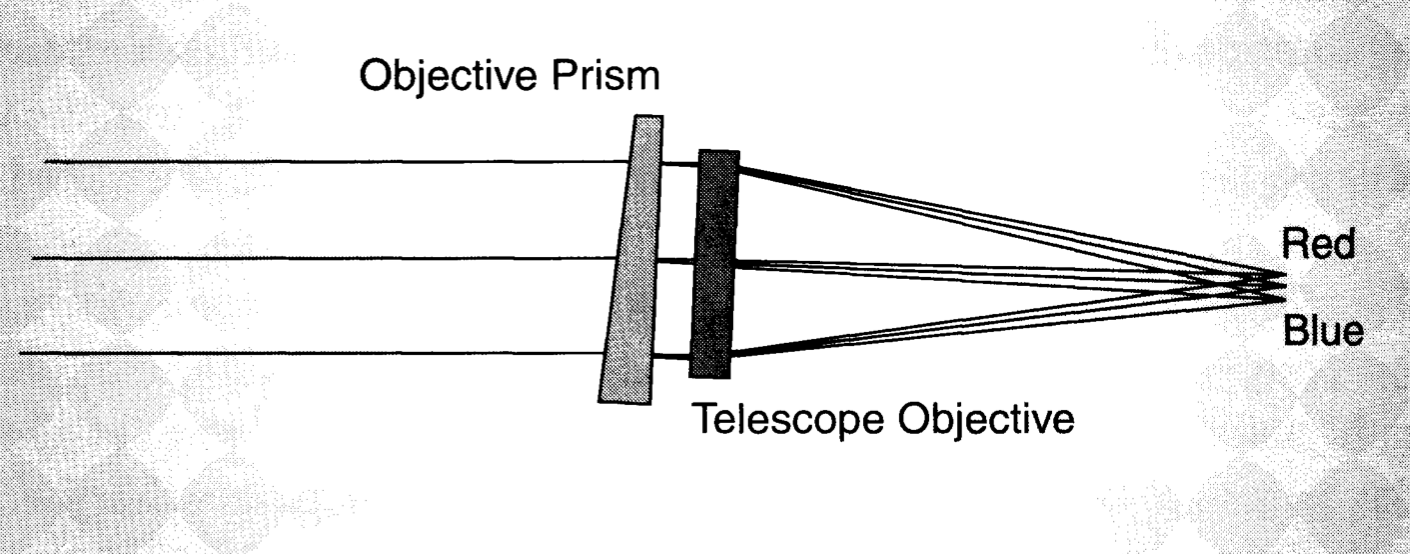
\includegraphics[scale=0.35]{Images/AsImages/S1/PRISM.png}
  \caption{\label{Prism}Illustration of the objective prism spectrograph operating in front of a telescope. Source (\cite{ImageProcessing}).}
\end{figure}
\begin{figure}[H]
  \centering
  \ContinuedFloat
  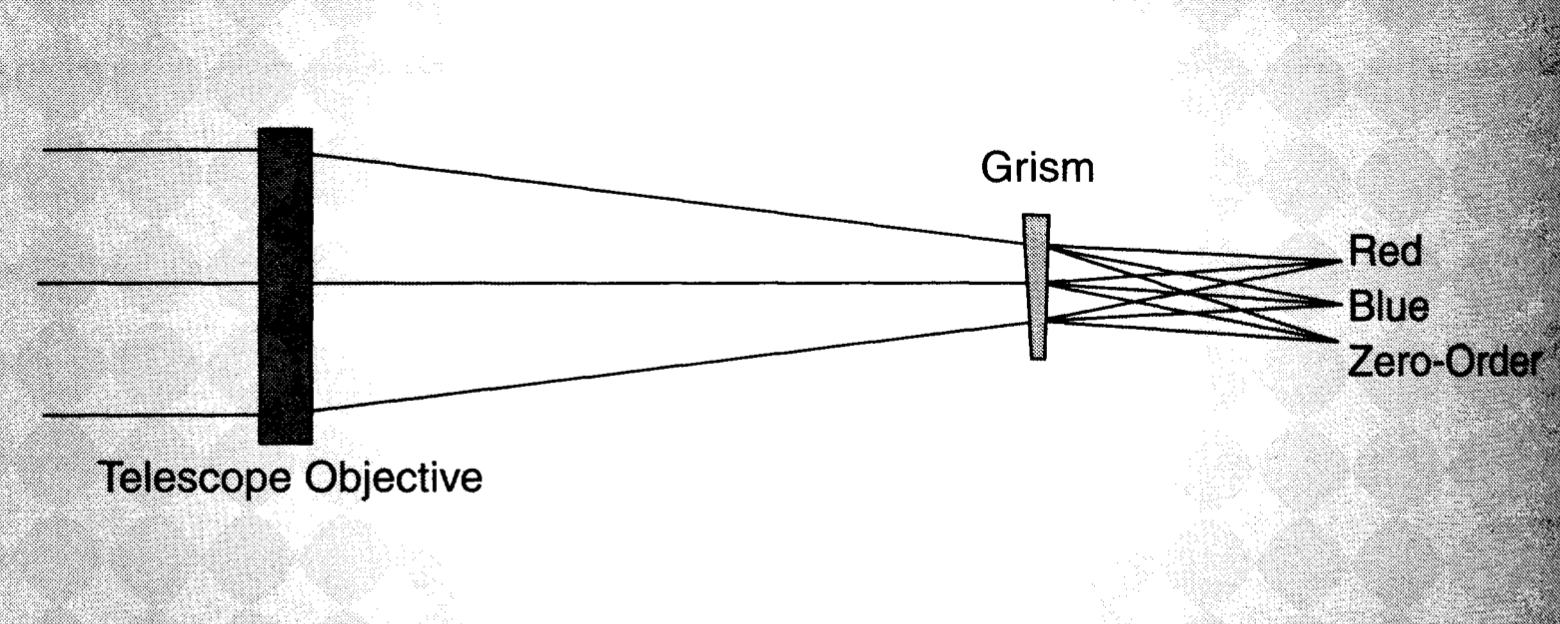
\includegraphics[scale=0.315]{Images/AsImages/S1/GRISM.png}
  \caption{\label{Grism}Illustration of the grating-prism (grism) spectrograph operating behind the telescope. Source (\cite{ImageProcessing}).}
\end{figure}
\end{multicols}

\noindent There are 4 types of spectrographs: The objective prism in \cref{Prism} sits in front of the telescope so the refractive index of glass separates all the light into wavelengths as they exit the prism, this is mostly used as its used to survey stars faster. The grating-prism (grism) in \cref{Grism} sits behind the telescope lense and refracts the light into wavelengths, this operation is cheaper as it operates 'diffraction grating'. The slit is place in front of the telescope and isolates the celestial body, thus narrows the light emitted for a prism/ grism to operate, the last is fiber-fed that allows the light to travel through optical glass fibers to the prism/grism separate from the telescope (\cite{ImageProcessing}).

%---------------------------------------------------------------------------
%	SECTION 2
%---------------------------------------------------------------------------
\section{Dispersion \& Resolving Power}
\label{Section 2}

Some properties of the spectrum/ spectra are dispersion and resolving power (spectral resolution). Dispersion is the light that diffracts off a prism/ grism and disperses into wavelengths, its simply the rate of change of the wavelength in relation to the spectrum distance, it can be computed into nanometers per pixel: 

\begin{equation}
\centering
\textnormal{Dispersion} = \textnormal{D}= \dfrac{\textnormal{Free Spectral Range}}{\textnormal{Number of Pixels}} \hspace{0.5cm }\textnormal{[nm/pixel]}
\label{Dispersion Equation}
\end{equation} \\ [-0.5cm]

\noindent Where the 'Free Spectral Range' is the wavelength range in the relevant spectrum: short-wavelengths of 360nm, ultraviolet wavelengths of 1100nm, infrared wavelengths of 740nm but and for stellar spectral objects at 150nm. The resolving power is a mixture of factors that separate lines which have a small difference in wavelength, such factors include: width of the slit, size of the star image, the fiber tip and the dispersion of the prism, grating and quality of the optics used (\cite{ImageProcessing}). Its computed by: 

\begin{equation}
\centering
\textnormal{Resolving Power} = \textnormal{R} = \dfrac{\textnormal{Wavelength}}{\textnormal{Resolution}} \hspace{0.5cm }\textnormal{[Dimensionless]}
\label{Resolving Power Equation}
\end{equation} \\ [-0.5cm]

\noindent The resolving power is most commonly twice that of the dispersion, its used to classify star types between 150 and 100 resolving power, whereas professional astronomers used a resolving powers up to 100,000 (\cite{ImageProcessing}). 

%---------------------------------------------------------------------------
%	SECTION 3
%---------------------------------------------------------------------------
\section{Spectroscopy Method}
\label{Section 3}

Using the 'spectroscopy tool' in the AIP4WIN software on the image file 'VegaSpectrum.fts' of a zero magnitude type A0V star Vega which was captured using a 6-inch objective prism, the image is already calibrated through dark frame subtraction and flat-fielding (\cite{ImageProcessingTutorial}).

\begin{figure} [H]
  \centering
  \ContinuedFloat*
  
\includegraphics[scale=0.93]{Images/AsImages/S3/VegaImage.PNG}
  \caption{\label{Vega Image}Infrared image of the Vega ready to undergo spectroscopy, \\ loaded into AIP4WIN software under 'VegaSpectrum.fts'.}
\end{figure}
\vspace{-0.5cm}
\begin{figure}[H]
  \centering
  \ContinuedFloat
  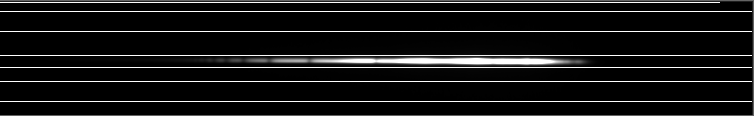
\includegraphics[scale=0.93]{Images/AsImages/S3/VegaSpectrum.PNG}
  \caption{\label{Vega Spectrum}Infrared image of Vega with the spectroscopic above sky, spectrum \\ and the bottom sky boundaries marked on 'VegaSpectrum.fts'.}
\end{figure}

By invoking the spectroscopy tool in \cref{Vega Spectrum Settings}, six boundary positions are plotted: two around the actual spectral region and the other four (two above and two below the spectral object) measuring the sky background. The 'objective mode' is selected as it takes a median of sky background across the entire image and this median is subtracted against the spectral object to further isolate the emitted light only from the spectral object. To set the 'vertical scale type' as linear to produce a set valued graph as seen in \cref{Vega Spectrum Settings}, pressing 'Save' gives a tabular of data which is used to produce the graph in \cref{Vega Spectrum Settings} and reproduce to provide more detail as seen in \cref{Vega Spectrum Graph}. As the image (\cref{Vega Spectrum Graph}) shows a horizontal profile of light of the Vega star (\cref{Vega Image}), it shows the intensity of light in relation to the the position of the star. It plots the light intensity as the pixel value from one side to the other while measuring the counts of intensity. The pixel value can be changed into wavelength using a calibration graph that measuring wavelength value instead of pixel value but by comparing  the peaks of data, its possible to match the pixel value to wavelength value and therefore find the type of light it emits from the electromagnetic light spectrum.

\newpage
\begin{multicols}{2}
\begin{figure}[H]
  \centering
  \ContinuedFloat*
  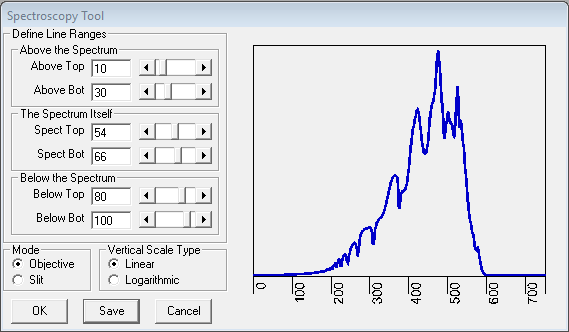
\includegraphics[scale=0.65]{Images/AsImages/S3/SpectrumSettings.PNG}
  \caption{\label{Vega Spectrum Settings}AIP4IWIN 'spectroscopy tool' above sky, spectrum and the bottom sky boundary \\ settings for \cref{Vega Spectrum} and its spectroscopic graph.}
\end{figure}
\begin{figure}[H]
  \centering
  \ContinuedFloat
  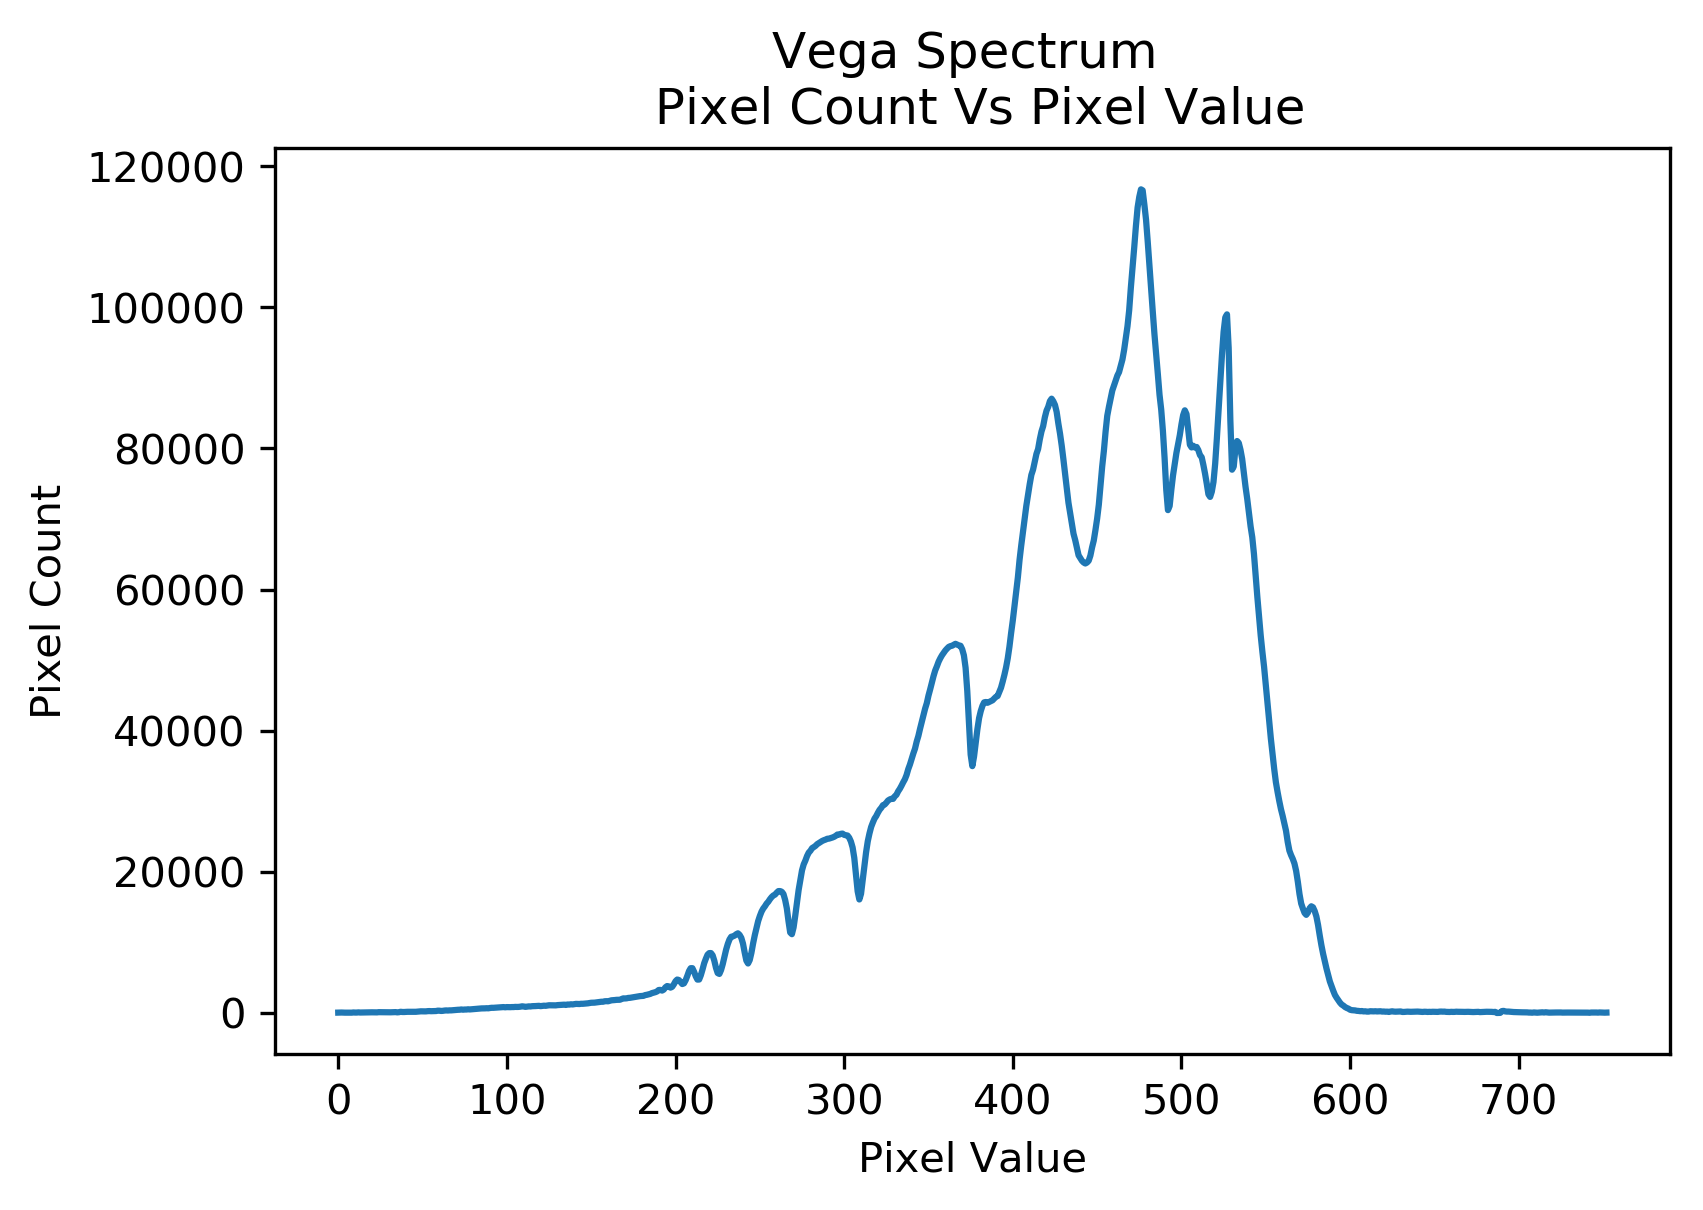
\includegraphics[scale=0.6]{Images/AsImages/S3/VegaPythonGraph.png}
  \caption{\label{Vega Spectrum Graph}Python reconstruction of the Vega spectrum graph in \cref{Vega Spectrum Settings}, showing the \\ individual pixel counts for each spectroscopic pixel value.}
\end{figure}
\end{multicols} 

%---------------------------------------------------------------------------
%	SECTION 4
%---------------------------------------------------------------------------
\section{Asteroid Spectroscopy}
\label{Section 4}
%---------------------------------------------------------------------------
\subsection{Asteroid Spectroscopy}
\label{SubSection 4a}

By obtaining the image files 'AST\_rot\_tr.fits', 'HeAr\_rot\_tr.fits' and 'SA\_rot\_tr.fits' and utilizing the spectroscopy method outlined in \cref{Section 3}, the spectroscopic boundaries were set for each image as seen in the figure 4a,b,c and as tabulated in \cref{Spectrum Settings}. Which the spectroscopic data was retrieved and it was plotted in figure 5a,b,c. As the 'HeAr\_rot\_tr.fits' image (\cref{HeAr Spectrum}) has no sky background subtraction as the captured spectrum is vertical in nature and thus will provide a fluctuating light profile. The 'SA\_rot\_tr.fits' image (\cref{SA Spectrum}) is the same image to that of the 'AST\_rot\_tr.fits' image (\cref{AST Spectrum}) but it is captured by placing a slit in front of the telescope and blocks out all the sky background. \\

\begin{table}[H]
\begin{center}
 \footnotesize
 \begin{tabular}{|c||c|c||c|c||c|c|}
 \hline
 \multicolumn{7}{|c|}{AIP4IWIN 'spectroscopy tool' above sky, spectrum and bottom sky boundary settings} \\
 \hline \hline
 Spectrum & \multicolumn{2}{|c||}{'AST\_rot\_tr.fits'} & \multicolumn{2}{c||}{'HeAr\_rot\_tr.fits'} & \multicolumn{2}{c|}{'SA\_rot\_tr.fits'} \\
 \hline
 Setting & Top & Bottom & Top & Bottom & Top & Bottom \\
 \hline \hline
 Above & 100 & 120 & 223 & 243 & 330 & 350 \\
 \hline
 Spectrum & 0 & 0 & 200 & 220 & 0 & 0 \\
 \hline
 Below & 90 & 110 & 223 & 243 & 330 & 350 \\
 \hline
 \end{tabular} \\ 
 \caption{AIP4IWIN 'spectroscopy tool' above sky, spectrum and the \\ bottom sky boundary settings for \cref{AST Spectrum}, \cref{HeAr Spectrum} and \cref{SA Spectrum}.}
 \label{Spectrum Settings}
\end{center}
\end{table} 

\newpage
\begin{multicols}{3}
\centering
\begin{figure} [H]
  \centering
  \ContinuedFloat*
  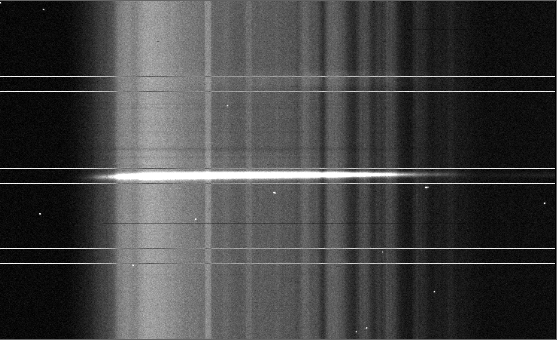
\includegraphics[scale=0.4]{Images/AsImages/S4/AST/AST_Spectrum.PNG}
  \caption{\label{AST Spectrum} 'AST\_rot\_tr.fits' image with it's spectroscopic boundaries valued in \cref{Spectrum Settings}}
\end{figure}
\begin{figure}[H]
  \centering
  \ContinuedFloat
  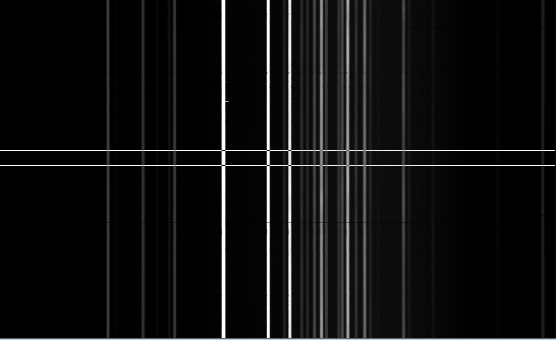
\includegraphics[scale=0.4]{Images/AsImages/S4/HeAr/HeAr_Spectrum.PNG}
  \caption{\label{HeAr Spectrum} 'HeAr\_rot\_tr.fits' image with it's spectroscopic boundaries valued in \cref{Spectrum Settings}}
\end{figure}
\begin{figure}[H]
  \centering
  \ContinuedFloat
  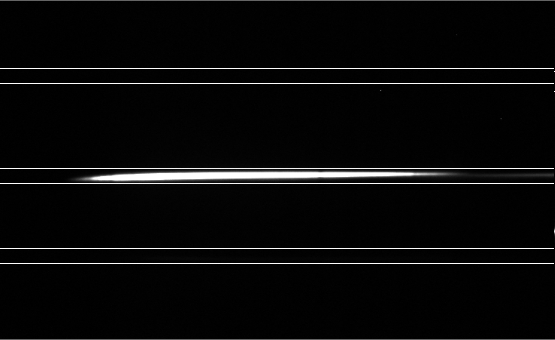
\includegraphics[scale=0.4]{Images/AsImages/S4/SA/SA_Spectrum.PNG}
  \caption{\label{SA Spectrum} 'SA\_rot\_tr.fits' image with it's spectroscopic boundaries valued in \cref{Spectrum Settings}}
\end{figure}
\end{multicols}

\begin{multicols}{3}
\centering
\begin{figure} [H]
  \centering
  \ContinuedFloat*
  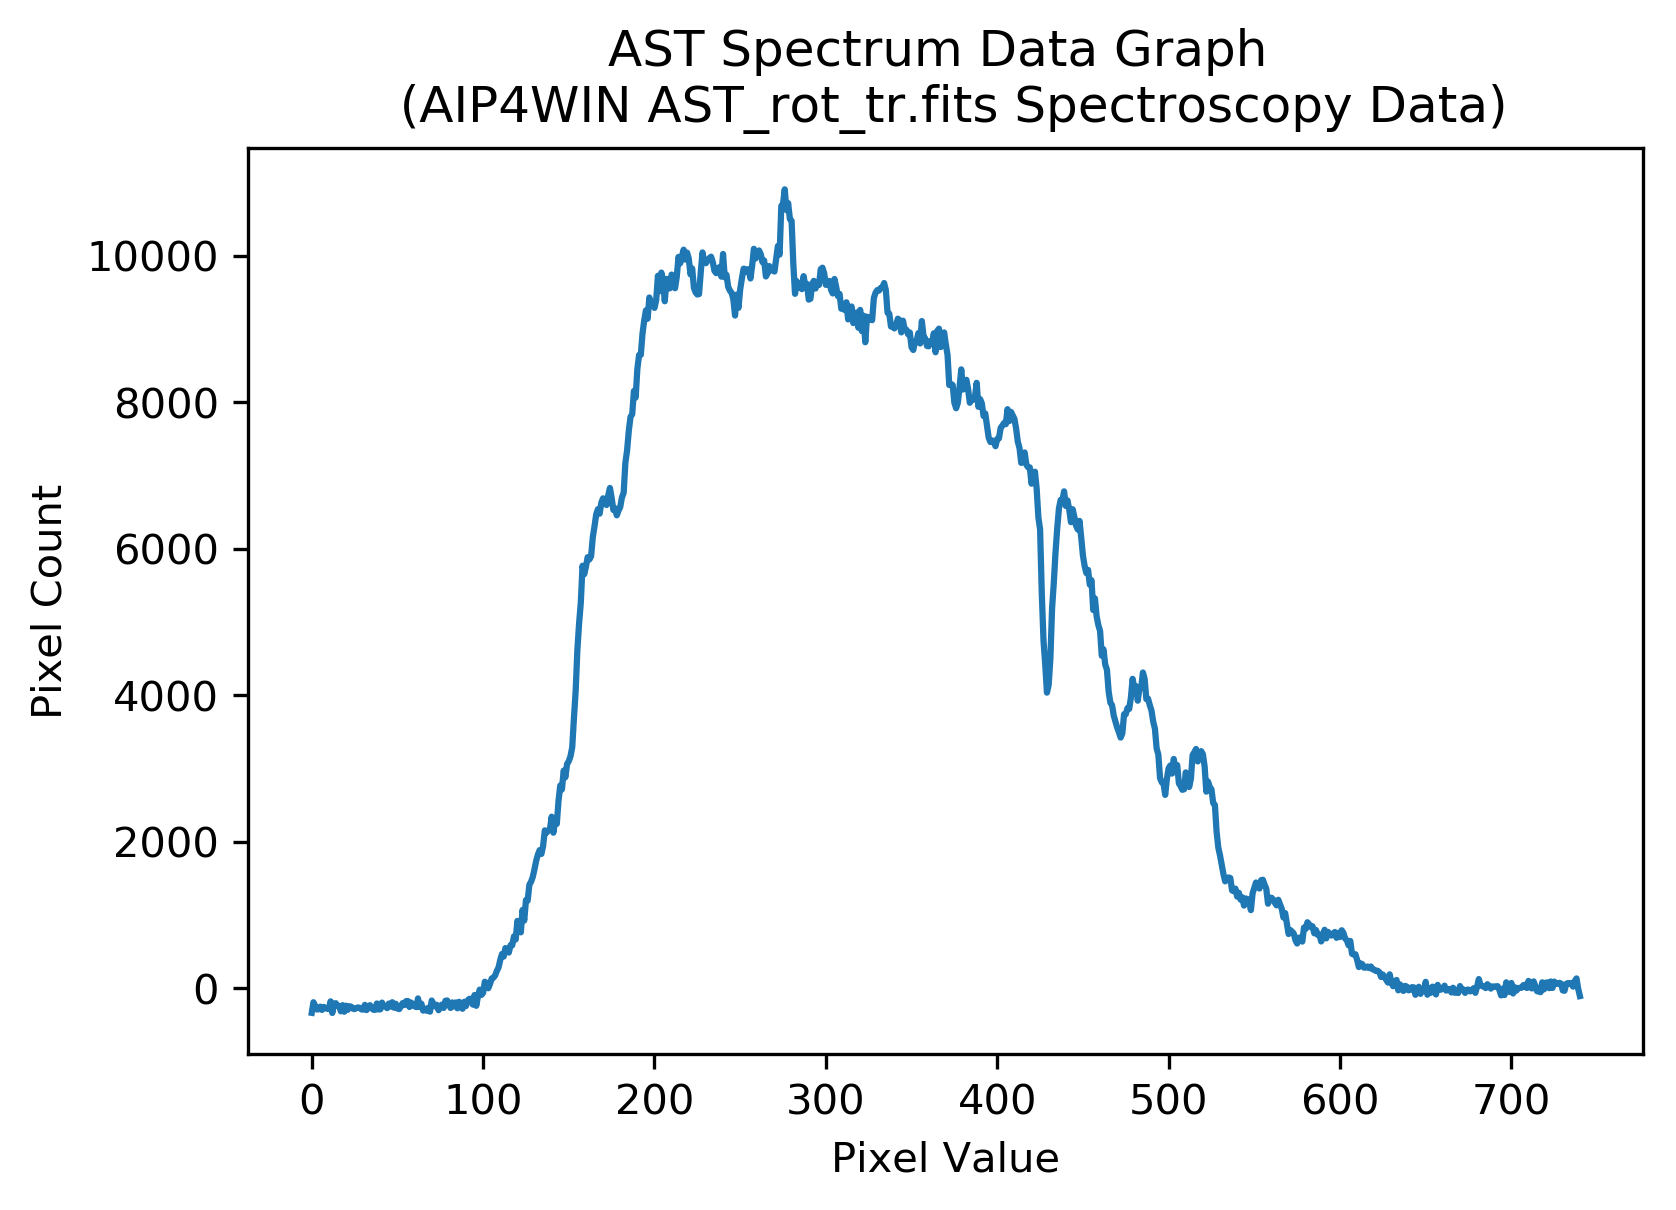
\includegraphics[scale=0.4]{Images/AsImages/S4/AST/ASTPythonGraph.png}
  \caption{\label{AST Python Graph} Graphical {'AST\_rot\_tr.fits'} spectroscopy data.}
\end{figure}
\begin{figure}[H]
  \centering
  \ContinuedFloat
  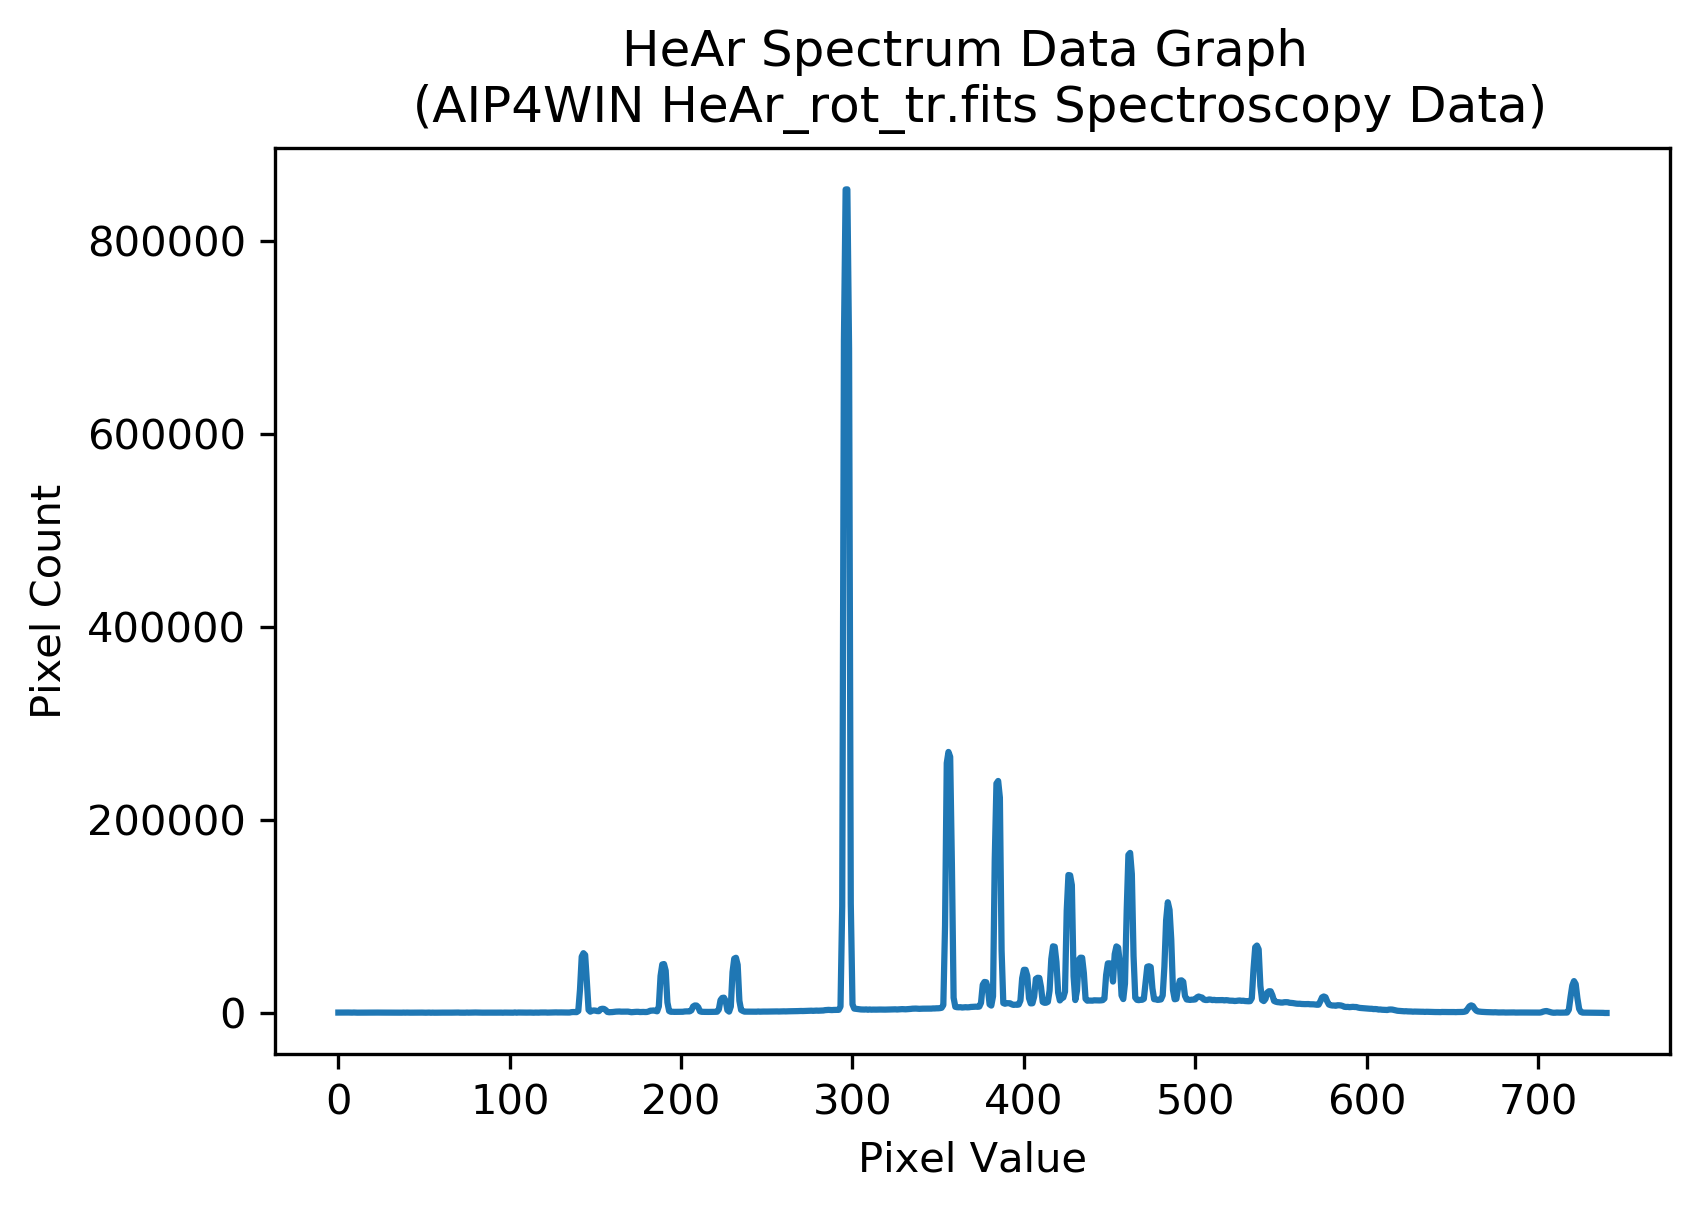
\includegraphics[scale=0.4]{Images/AsImages/S4/HeAr/HeArPythonGraph.png}
  \caption{\label{HeAr Python Graph} Graphical 'HeAr\_rot\_tr.fits' spectroscopy data.}
\end{figure}
\begin{figure}[H]
  \centering
  \ContinuedFloat
  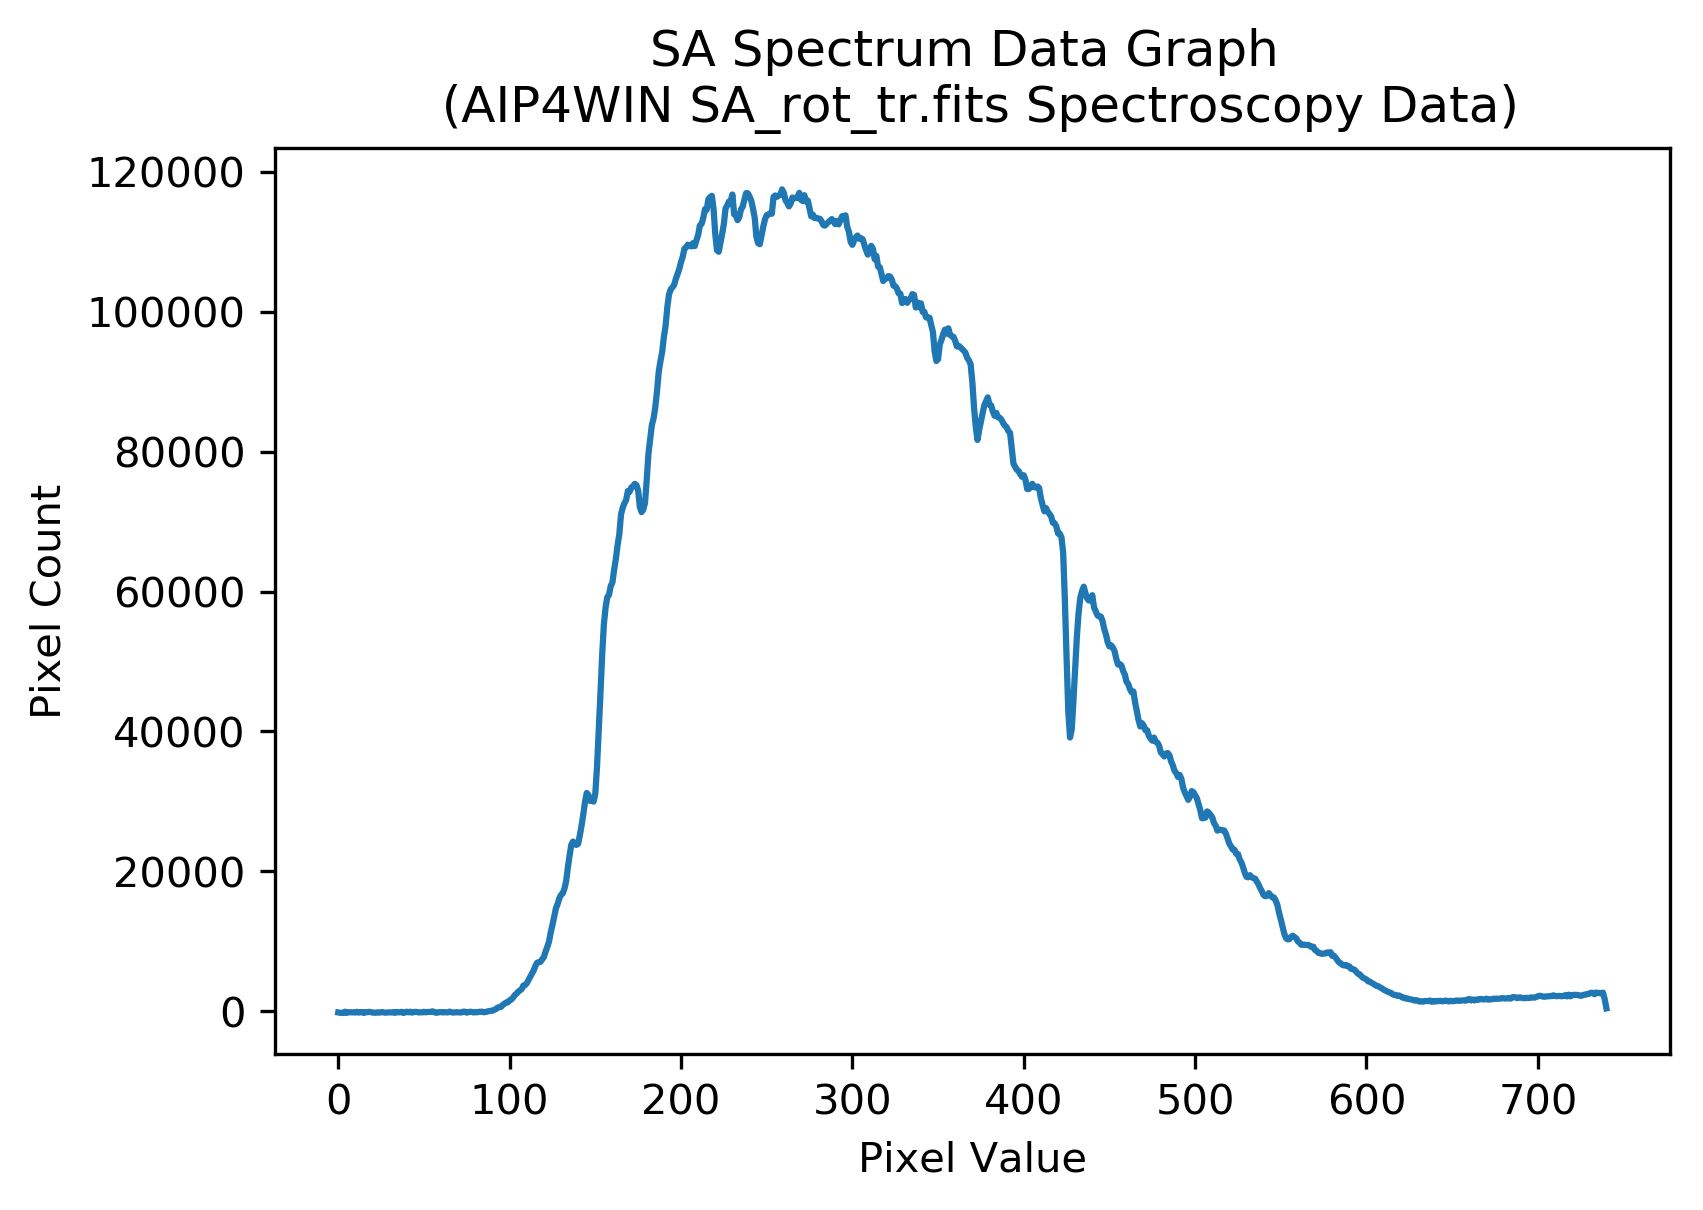
\includegraphics[scale=0.4]{Images/AsImages/S4/SA/SAPythonGraph.png}
  \caption{\label{SA Python Graph} Graphical 'SA\_rot\_tr.fits' \\spectroscopy data.}
\end{figure}
\end{multicols}

%---------------------------------------------------------------------------
\subsection{Asteroid Calibration}
\label{SubSection 4b}

A calibration is in order to relate the pixel values with wavelength, this is achieved by physically comparing a set data graph seen in \cref{HeAr Cali Graph} with the experimental data graph resourced in \cref{SubSection 4a}. The calibration is tabulated in \cref{Calibration Data}, where the wavelength in angstrom (\si{\angstrom}) is converted to nanometres (nm) by the definition of 10\si{\angstrom} = 1nm (\cite{ImageProcessing}).

\begin{multicols}{2}
\begin{figure}[H]
  \centering
  \ContinuedFloat*
  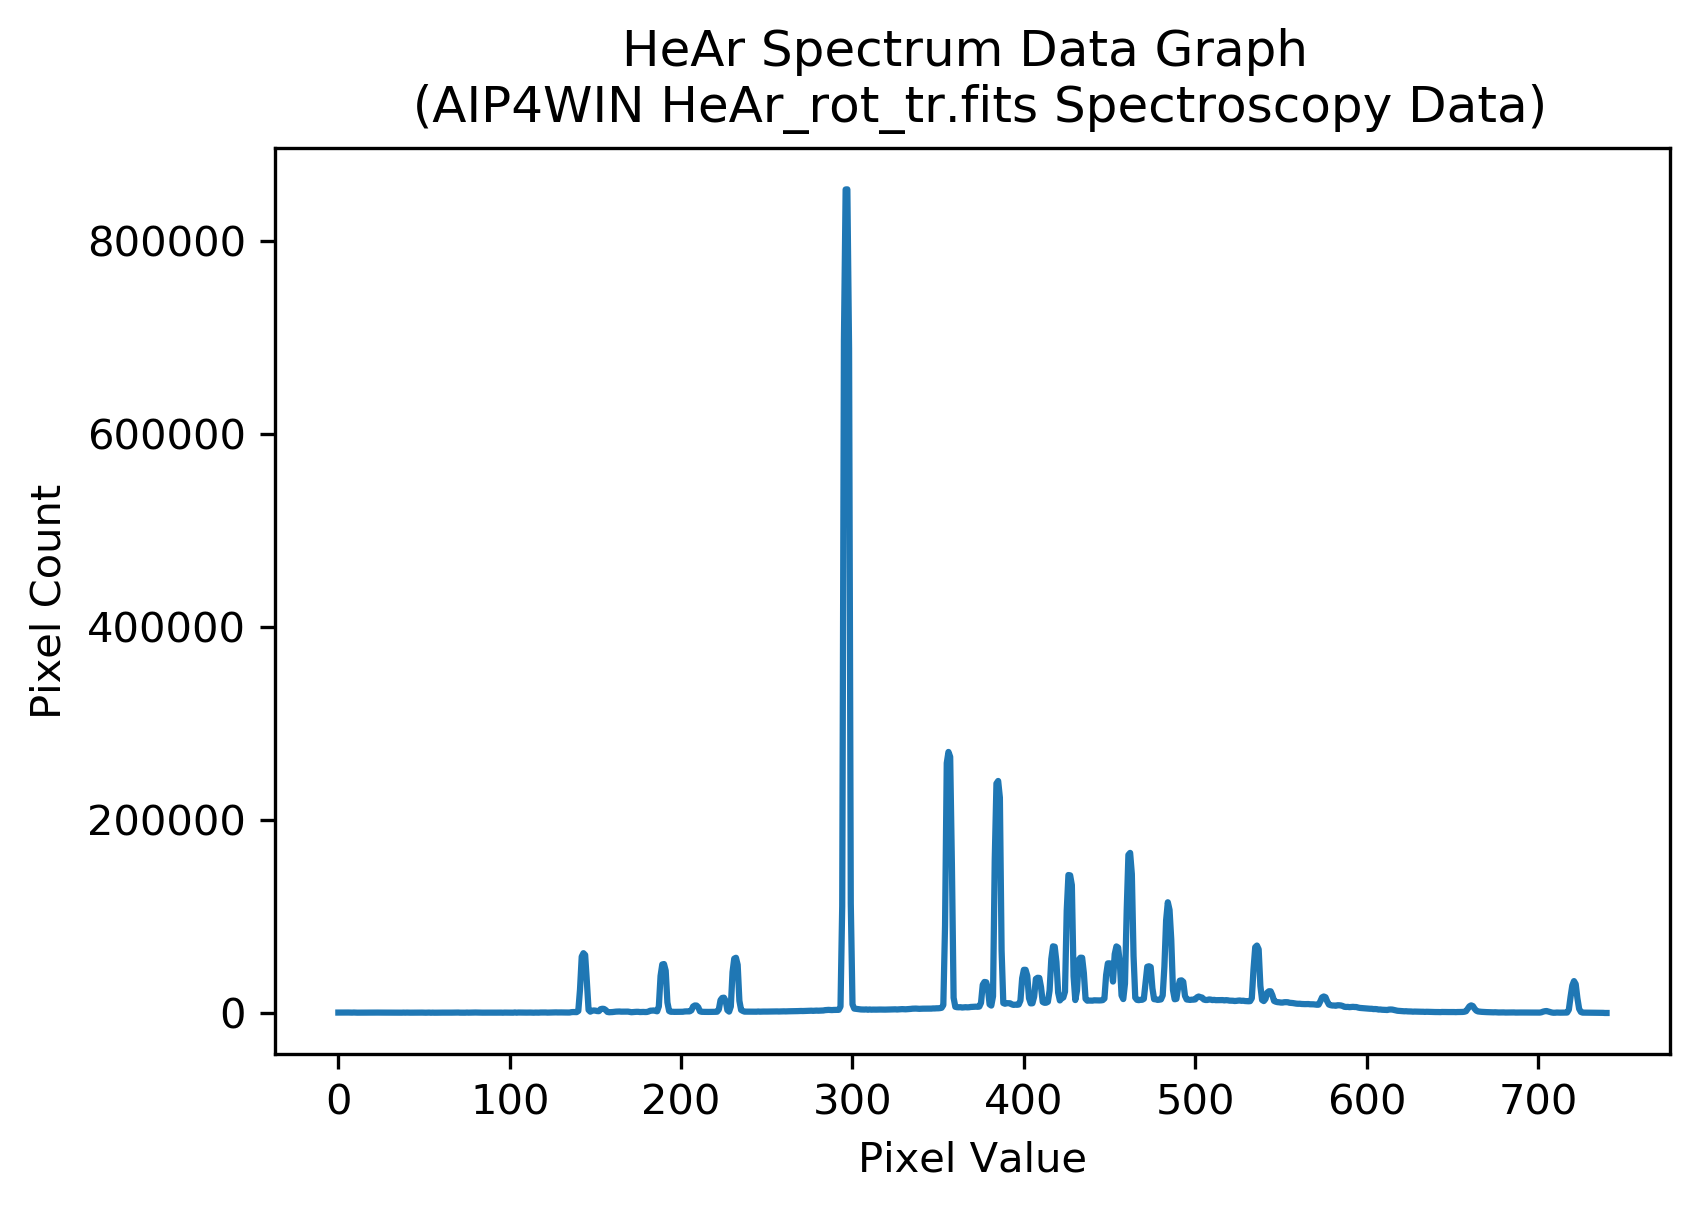
\includegraphics[scale=0.6]{Images/AsImages/S4/HeAr/HeArPythonGraph.png}
  \caption{\label{HeAr Cali Python Graph} Graphical 'HeAr\_rot\_tr.fits' spectroscopy data.}
\end{figure}
\begin{figure}[H]
  \centering
  \ContinuedFloat
  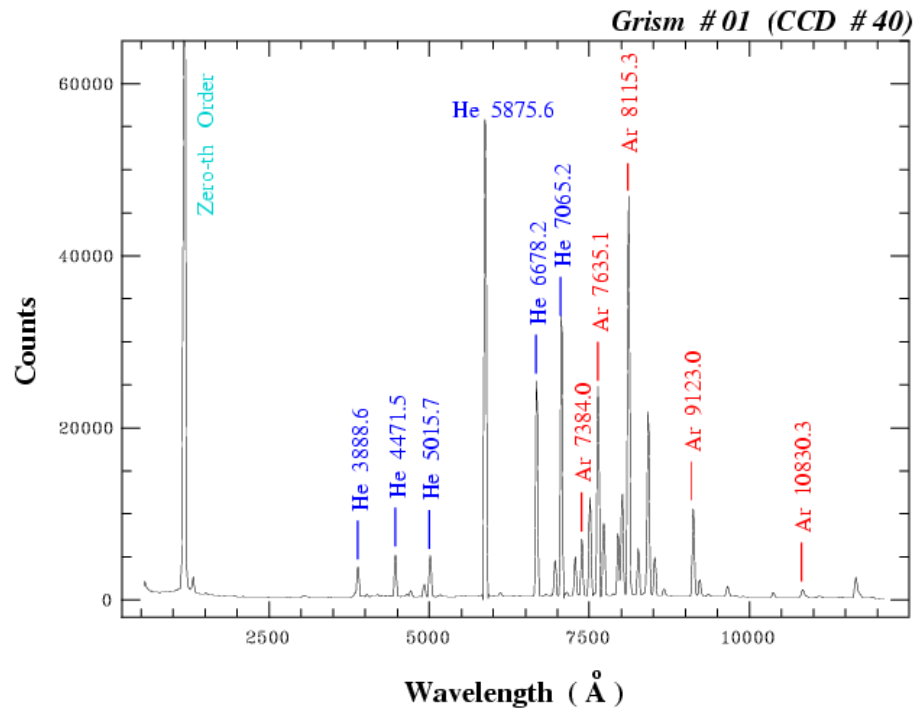
\includegraphics[scale=0.35]{Images/AsImages/S4/HeAr/He-Ar_Arc-Lamp_Spectrum.PNG}
  \caption{\label{HeAr Cali Graph} Calibration image for 'HeAr\_rot\_tr.fits' image.}
\end{figure}
\end{multicols}

\begin{table}[H]
\begin{center}
 \footnotesize
 \begin{tabular}{|c|c|c|c|c||c|c|c|c|c|}
 \hline
 \multicolumn{10}{|c|}{Calibration data of experimental and theory data } \\
 \hline \hline
 \multicolumn{5}{|c||}{Helium} & \multicolumn{5}{c|}{Argon} \\
 \hline
 Element & $\lambda$ (\si{\angstrom}) & $\lambda$ (nm) & Pixel Values & Spectrum & Element & $\lambda$ (\si{\angstrom}) & $\lambda$ (nm) & Pixel Values & Spectrum \\
 \hline \hline
 He 3888.6 & 3888.6 & 388.9 & 140 & UV & Ar 7384.0 & 7384.0 & 738.4 & 410 & IR \\
 \hline
 He 4471.5 & 4471.5 & 447.2 & 190 & Blue & Ar 7635.1 & 7635.1 & 763.5 & 425 & IR\\
 \hline
 He 5015.7 & 5015.7 & 501.2 & 230 & Green & Ar 8115.3 & 8115.3 & 811.5 & 485 & IR \\
 \hline
 He 5875.6 & 5875.6 & 587.6 & 295 & Yellow & Ar 9123.0 & 9123.0 & 912.3 & 530 & IR \\
 \hline
 He 6678.2 & 6678.2 & 667.8 & 355 & Red & Ar 10830.3 & 10830.3 & 1083.0 & 660 & IR\\
 \hline
 He 7065.2 & 7065.2 & 706.5 & 385 & IR & & & & & \\
 \hline
 \end{tabular} \\ 
 \caption{Calibration data of \cref{HeAr Cali Python Graph} and \cref{HeAr Cali Graph}, by comparing peaks to fix a wavelength to a pixel value.}
 \label{Calibration Data}
\end{center}
\end{table} 
\vspace{-0.5cm}

\noindent By associating the pixel value with a given wavelength, its now possible to specify on the experimental data graphs that at a certain pixel values equals to a certain wavelength. For example using \cref{Calibration Data} at a pixel value of 410, its wavelength value is 738.4nm. This now allows for comparison with the electromagnetic light spectrum to specify which type of light is at each individual pixel value by using \cref{EM Light Spectrum}. Thus as seen in \cref{Calibration Data} the spectrum type is shown as each element is categorised in each spectrum and each colour of the visible spectrum. \\ [-1.0cm]

\begin{figure}[H]
  \centering
  \ContinuedFloat*
  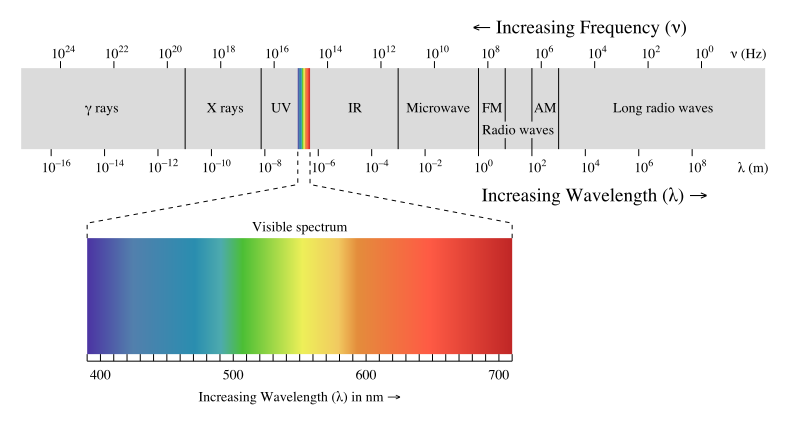
\includegraphics[scale=0.6]{Images/AsImages/S4/LightSpectrum.png}
  \caption{\label{EM Light Spectrum} Illustration of the electromagnetic spectrum (\cite{EM}).}
\end{figure}

By using the calibration of wavelength and or determining the wavelength per pixel in \cref{Poly Eq}, its seen that the 'Hear\_rot\_tr.fits' image (\cref{HeAr Python Graph}) emits in the yellow spectrum at its peak, whereas the 'AST\_rot\_tr.fits' image (\cref{AST Python Graph}) and the 'SA\_rot\_tr.fits' emits in the green spectrum. On a side note its possible to calculate the dispersion as the factors of \cref{Dispersion Equation} are known: 

\begin{equation}
\centering
\textnormal{Dispersion} = \textnormal{D}= \dfrac{\textnormal{Free Spectral Range}}{\textnormal{Number of Pixels}} \hspace{0.5cm } = \dfrac{150{\times10}^{-9}\textnormal{m}}{740 \hspace{0.1cm}\textnormal{Pixels}} = 0.203 \hspace{0.1cm} \textnormal{nm/pixel}
\label{Image Dispersion}
\end{equation} \\
\vspace{-0.5cm}

Its possible to calculate the resolving power as well for each individual wavelength using \cref{Resolving Power Equation} and taking the resolution of the telescope. \\

%---------------------------------------------------------------------------
\newpage
\subsection{Solar Analog Analysis}
\label{SubSection 4c}

By sourcing the data from \cref{AST Spectrum} and \cref{SA Spectrum} where instead of taking the objective and background sky light together and letting the software subtract it itself, they are taken separately where the background sky is subtracted against the objective is done manually. Using \cref{HeAr Cali Graph} its possible to find the best fitting polynomial which is specified as:

\begin{equation}
\centering
\lambda_i= a + b x_i 
\label{Poly Eq}
\end{equation} 

\begin{equation}
\centering
a = \lambda_i - (b x_i) \rightarrow 3888.6 - (13.53 * 143) = 1953.81
\label{Poly Eq a}
\end{equation} 

\begin{equation}
\centering
b = \dfrac{\lambda_2 - \lambda_1}{x_2 - x_1} \rightarrow \dfrac{9123.0 - 3888.6}{530 - 143} = 13.53
\label{Poly Eq b}
\end{equation} 
\vspace{0.5cm}

Using \cref{Poly Eq}, its possible to work out the wavelength per pixel ($\lambda_i$) and $x_i$ is pixel value where a and b are constants, this allows further analysis of the image in relation to the electromagnetic spectrum. To normalise the data shown in \cref{AST Cor Python Graph} and \cref{SA Cor Graph}, where the values of the highest peak of the graph was taken and the individual spectrum value on the data set was divided by this value at the highest peak, this will normalise the graph so the axis are all the same so the asteroid and the solar analog images can be accurately compared, the y-axis for both image were of different values where now they are the same. \\

\begin{multicols}{2}
\begin{figure}[H]
  \centering
  \ContinuedFloat*
  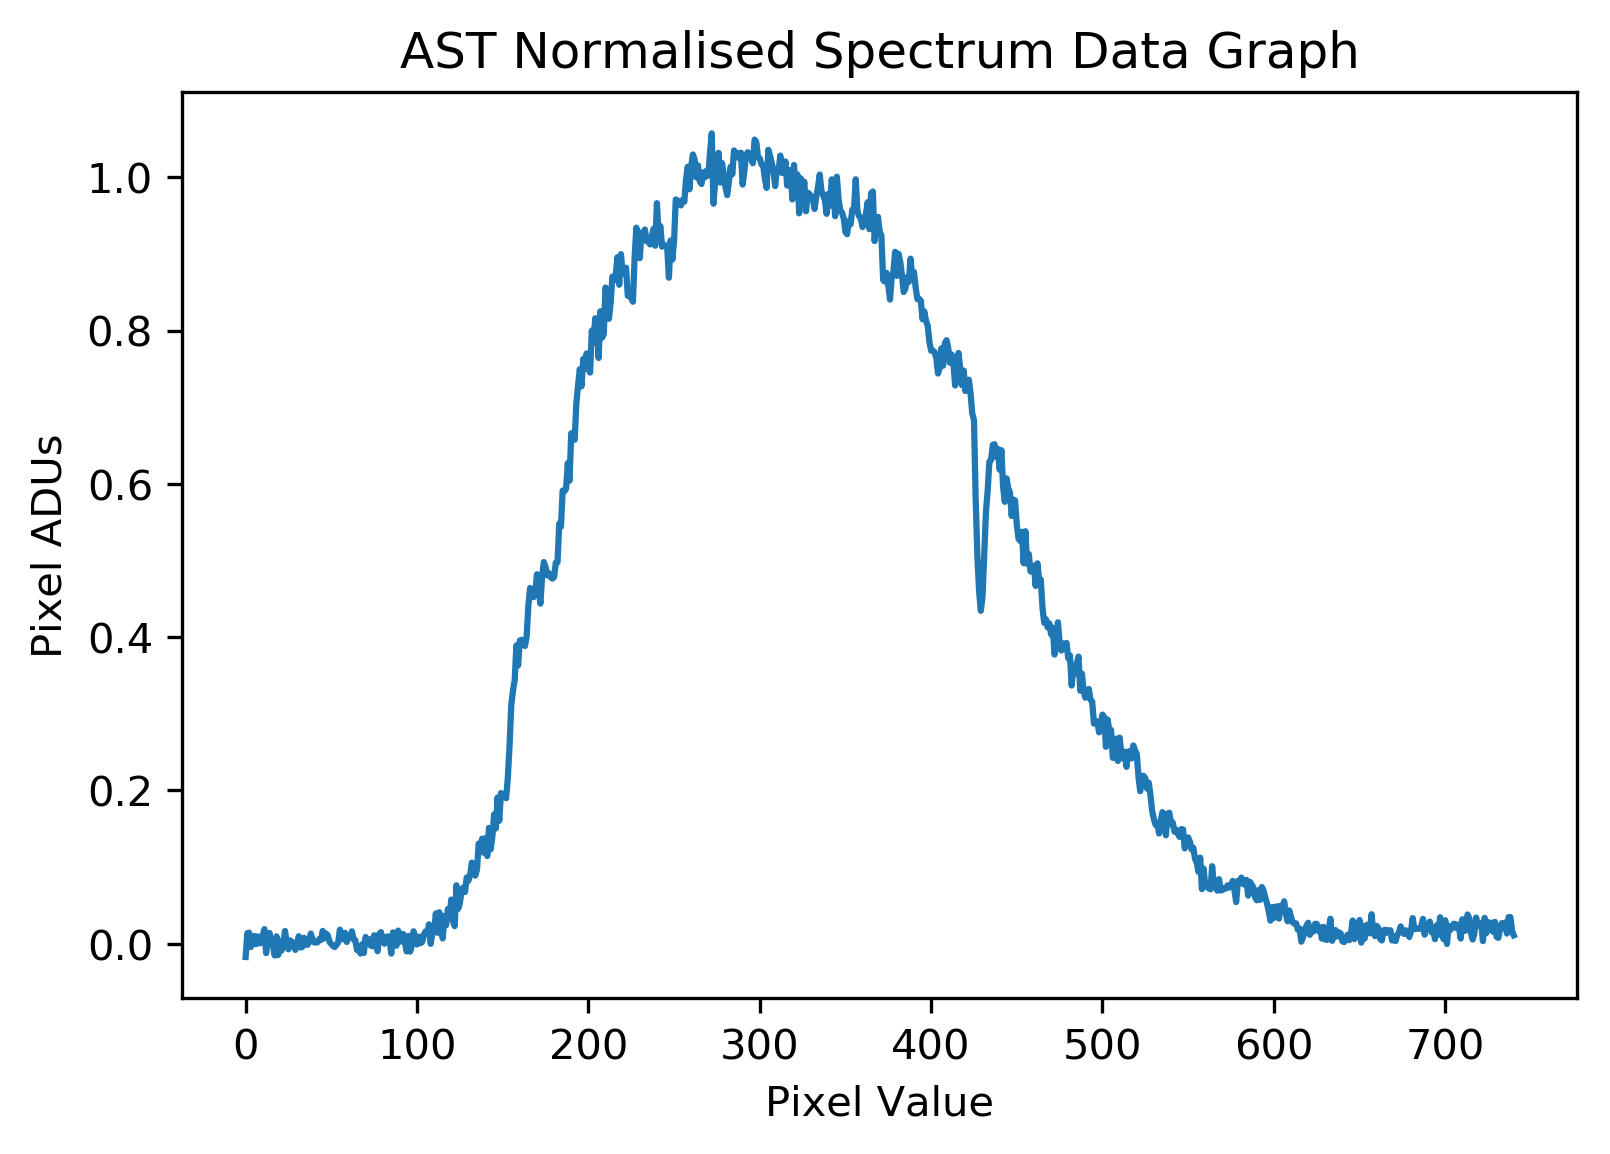
\includegraphics[scale=0.6]{Images/AsImages/S4/SC/ASTCorPythonGraph.png}
  \caption{\label{AST Cor Python Graph} Graphical 'AST\_rot\_tr.fits' normalised spectroscopy data.}
\end{figure}
\begin{figure}[H]
  \centering
  \ContinuedFloat
  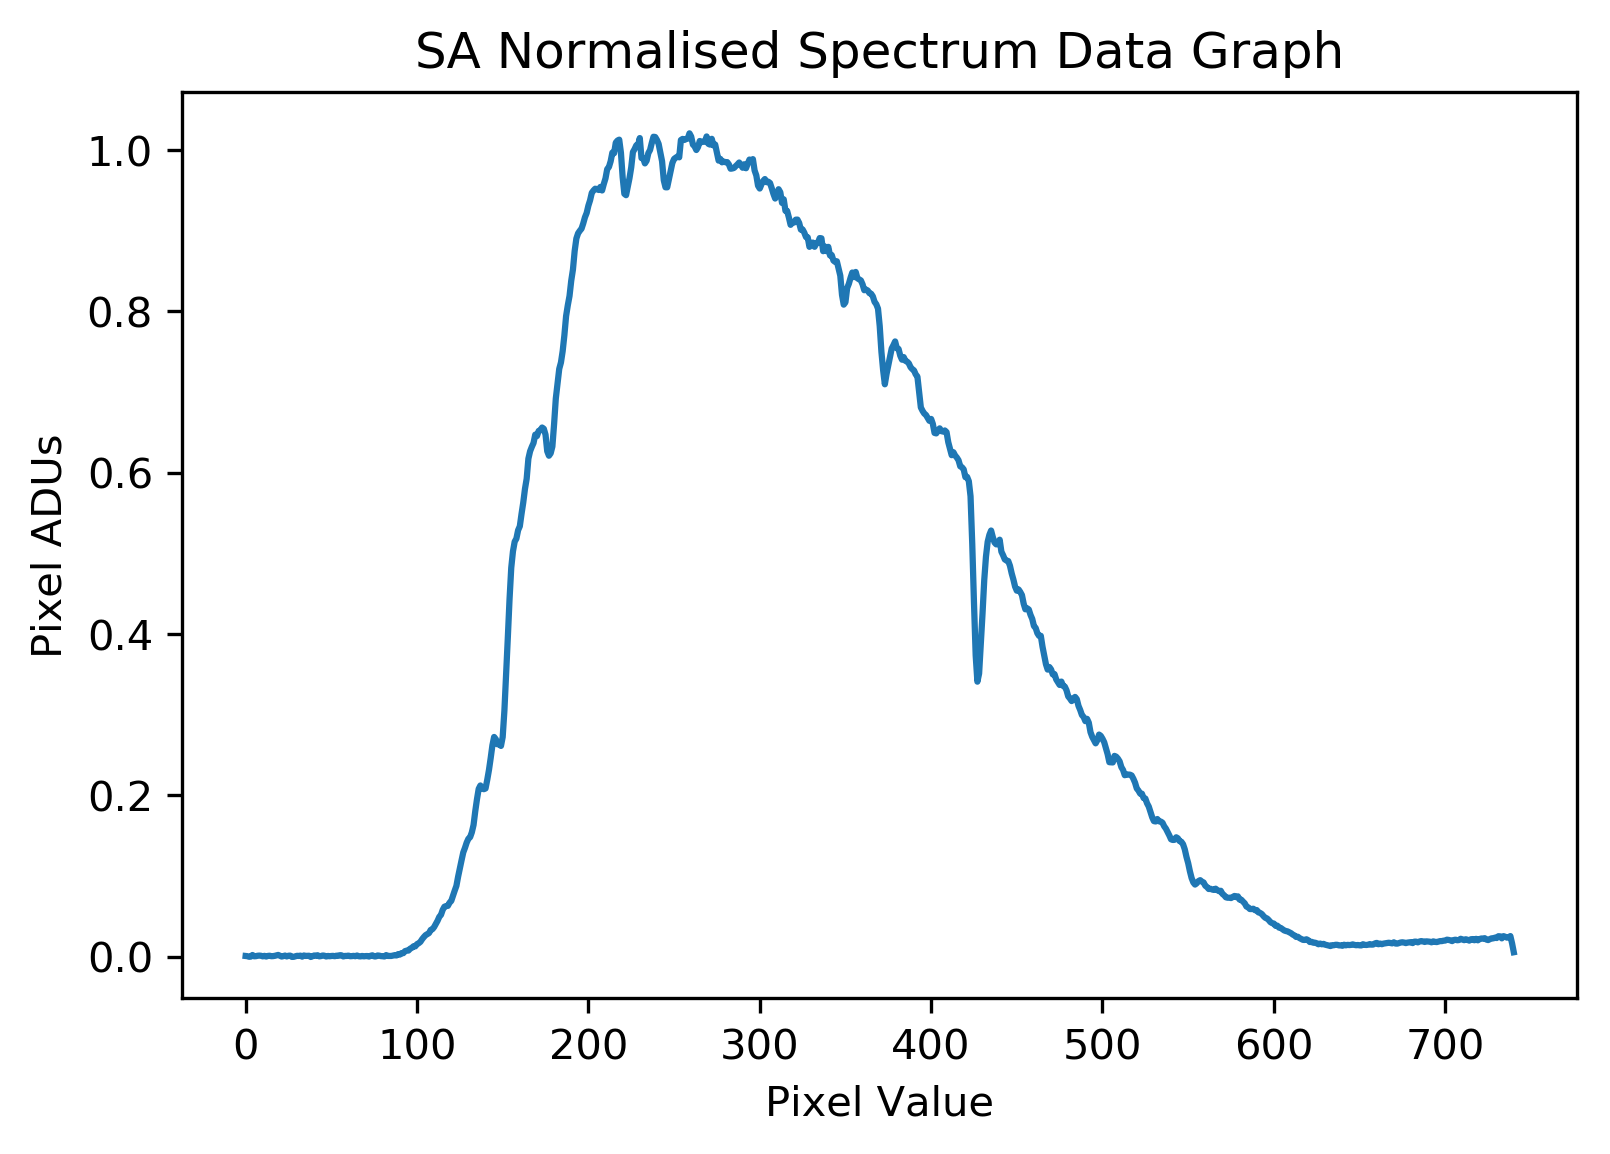
\includegraphics[scale=0.6]{Images/AsImages/S4/SC/SACorPythonGraph.png}
  \caption{\label{SA Cor Graph} Graphical 'SA\_rot\_tr.fits' normalised spectroscopy data.}
\end{figure}
\end{multicols}

The normalised data is plotted in \cref{AST Cor Python Graph} and \cref{SA Cor Graph} where the normalised will equal the axes where they can be plotted against each other in \cref{AST Vs SA Cor Python Graph}, as they have been normalised, comparing them becomes easier as it can be seen that the moving the slit of the telescope for the 'SA\_rot\_tr.fits' doesn't allow for background sky subtraction thus altering the data set between both the asteroid image and the solar analog image. By diving the solar analog data with the asteroid data, the difference in results is shown more in \cref{AST/SA Cor Graph}, this shows the difference in results between the using a slit and subtracting background sky counts. \\

\newpage
\begin{figure}[H]
  \centering
  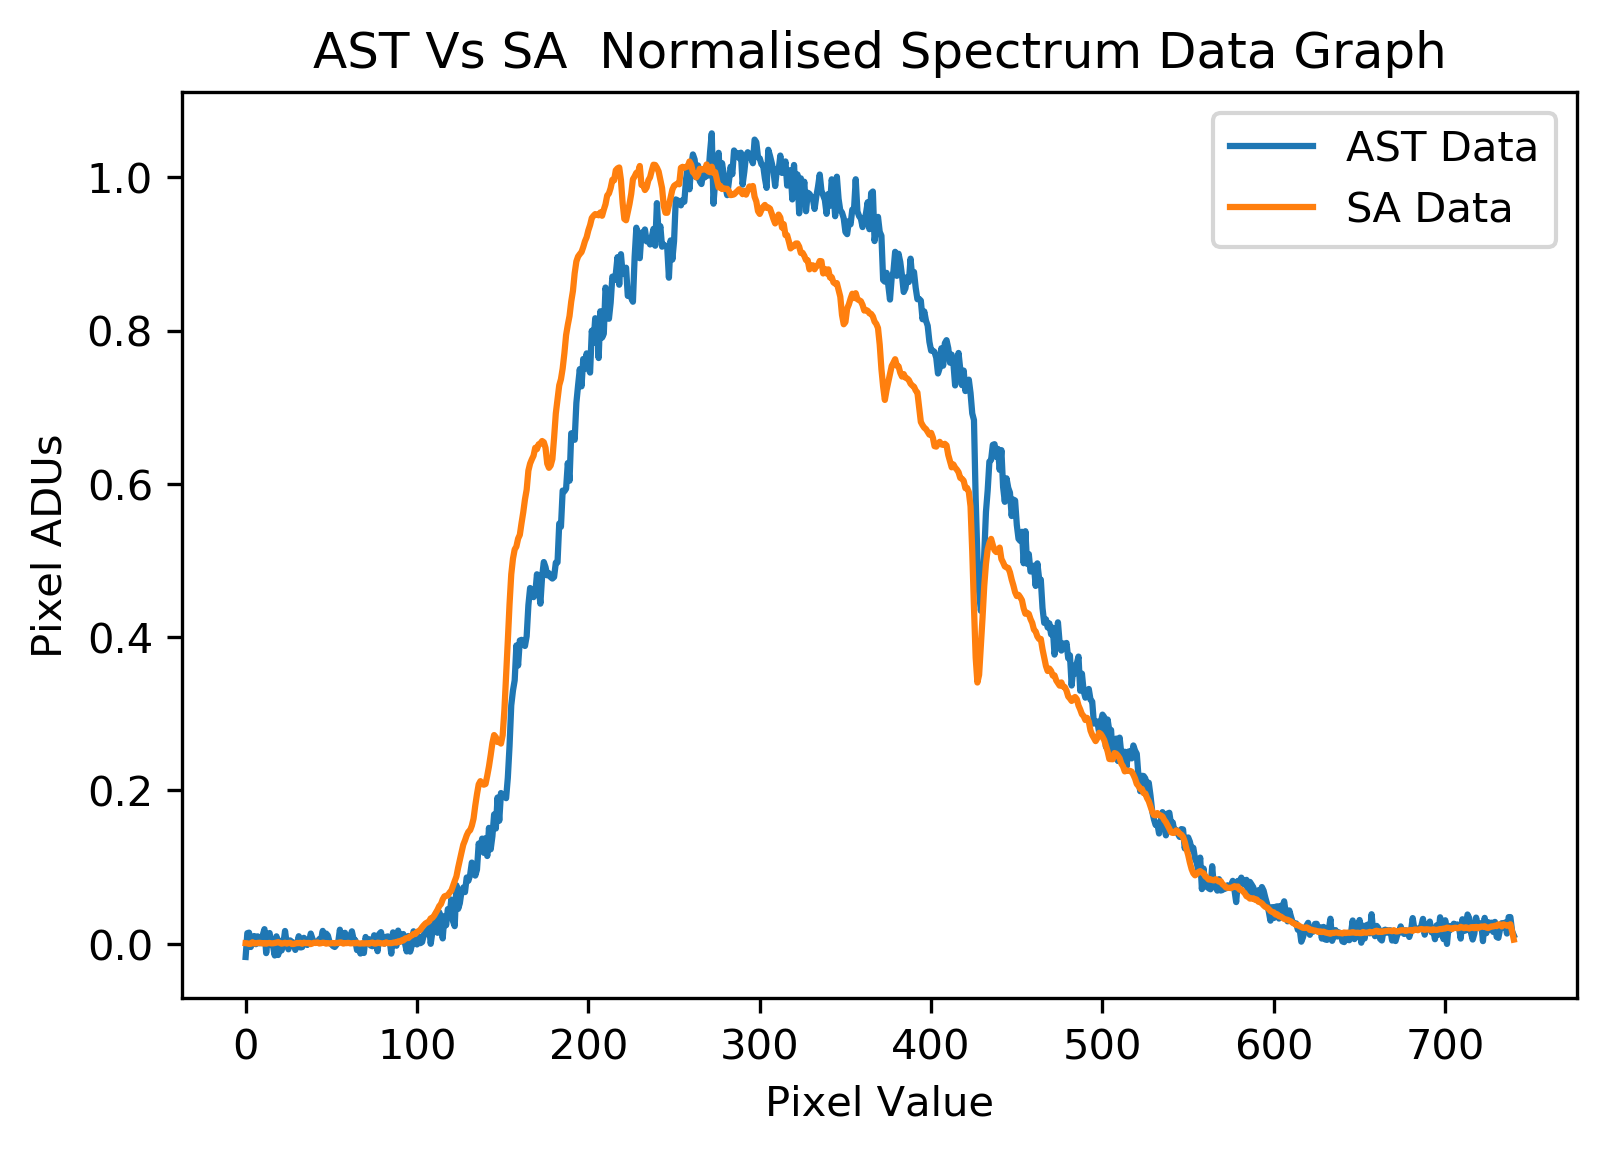
\includegraphics[scale=1.0]{Images/AsImages/S4/SC/ASTVsSAPythonGraph.png}
  \caption{\label{AST Vs SA Cor Python Graph} Graphical 'AST\_rot\_tr.fits' against 'SA\_rot\_tr.fits' normalised spectroscopy data.}
\end{figure}
\begin{figure}[H]
  \centering
  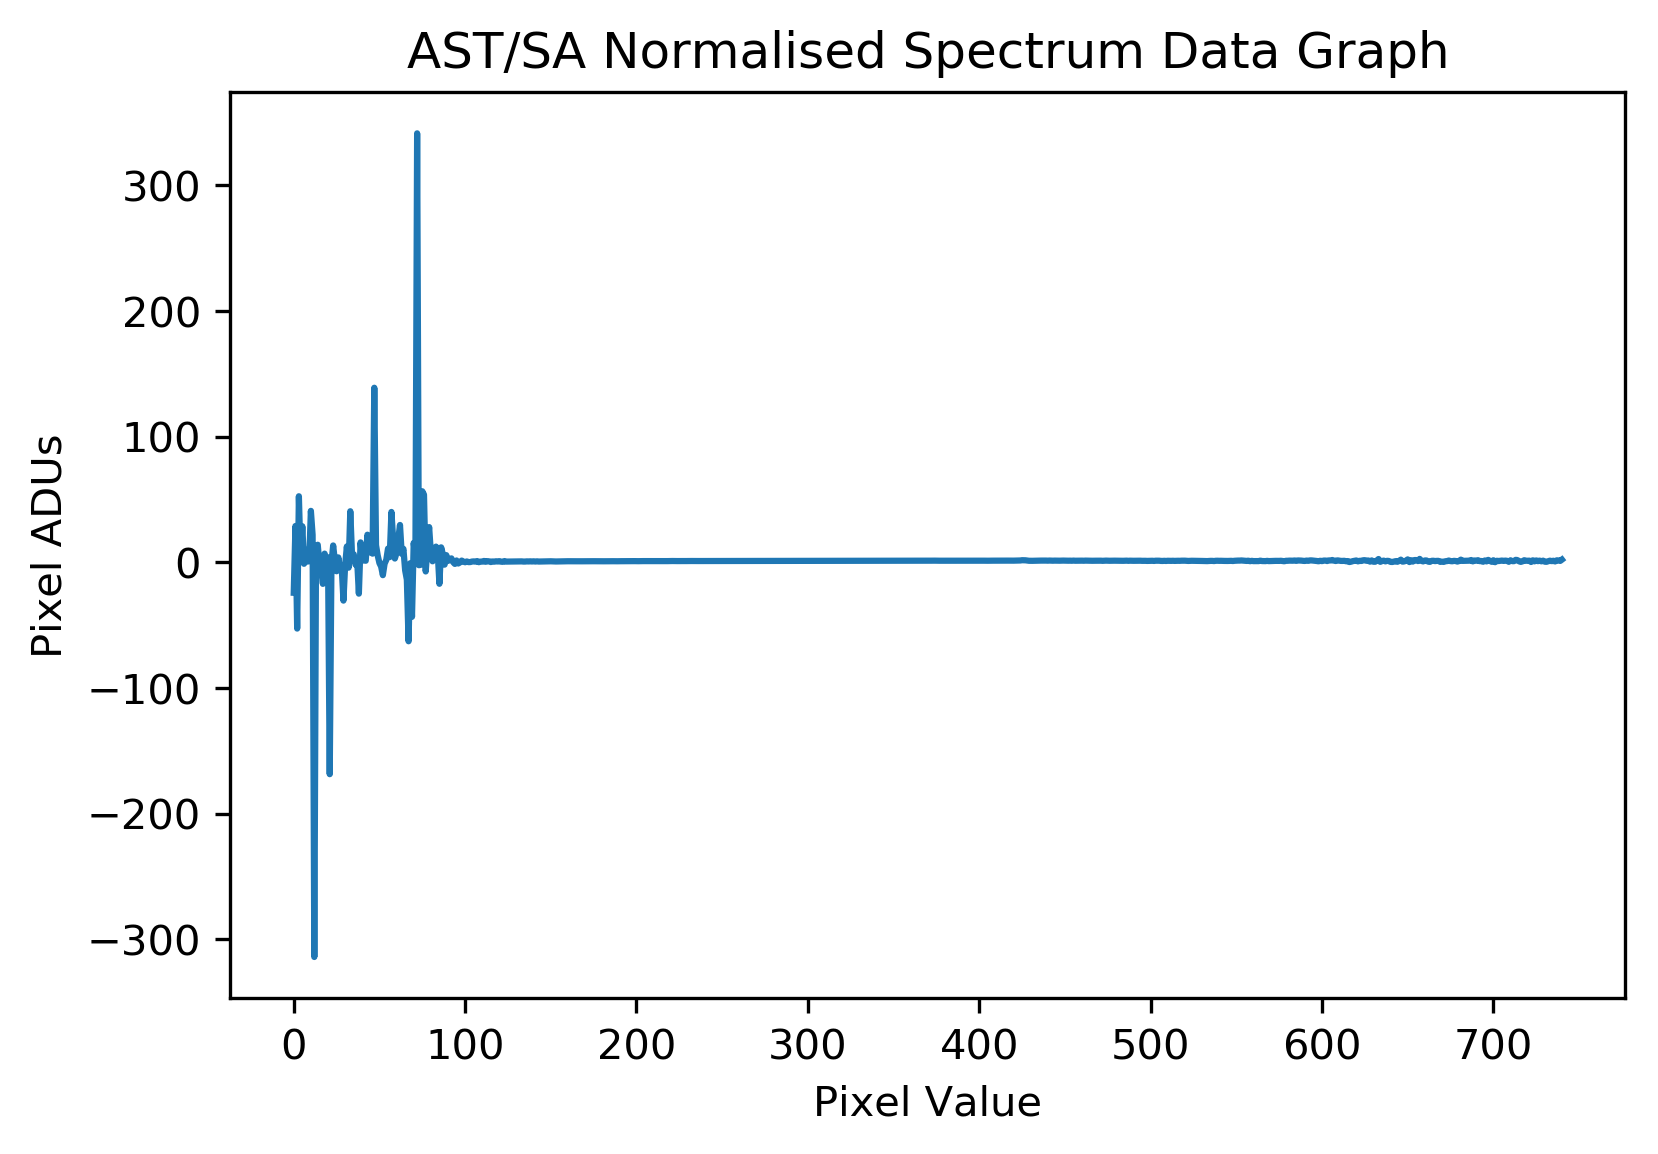
\includegraphics[scale=1.0]{Images/AsImages/S4/SC/AST-SAPythonGraph.png}
  \caption{\label{AST/SA Cor Graph} Graphical representation of the 'AST\_rot\_tr.fits' data divided by the 'SA\_rot\_tr.fits' data.}
\end{figure}

%---------------------------------------------------------------------------
\section{Asteroid Discussion}
\label{Section 5}

By using (\cite{Asteroids}) they used spectroscopy to determine the distribution of basaltic asteroids, they analysed and striped the data off each asteroid reported in the MOVIS-C catalogue from the Minor Planet center, all the data was normalised and three main types of meteorite's were compared with each other. They further went on to classify the distribution in terms of wavelength where they further used the data to determine the absolute magnitude of each basaltic asteroid. \\

The results in this report were normalised like in (\cite{Asteroids}), as to allow accurate comparison of multiple asteroids and provide further analysis of the difference between each asteroid in this experiment and or in (\cite{Asteroids}). This shows that not only can spectroscopy be used to determine the colour of the electromagnetic spectrum of the light emitted off the objective spectrum but through further analysis can help in astrometry and photometry. This proves that all of spectroscopy is another tool in the belt of image processing that continues to assist astronomers in observering the universe.

%---------------------------------------------------------------------------
\addcontentsline{toc}{section}{References}
\printbibliography
\end{document}